\documentclass{standalone}
\usepackage{tikz}
\usetikzlibrary{decorations.pathreplacing}
\begin{document}

            % TIKZ
            %$\left\{
                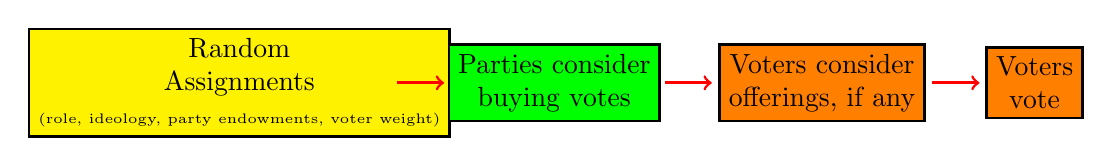
\begin{tikzpicture}[
                %scale=2
                scale=.2,
                line width=1pt] %

% random


                    % 1
                    \node[draw,align=center,fill=yellow,text=black] (RA) at (-22,-5.5) {Random\\Assignments\\\tiny{(role, ideology, party endowments, voter weight)}}; % 1
                    \path [red,  ->] (-12,-5.5) edge (-9,-5.5);


                    % 2
                    \node[draw,align=center,fill=green,text=black] (OFFERP) at (-2,-5.5) {Parties consider\\buying votes}; % 1
                    \path [red,  ->] (5,-5.5) edge (8,-5.5);

                    % 3
                    \node[draw,align=center,fill=orange,text=black] (OFFERV) at (15,-5.5) {Voters consider\\offerings, if any}; % 1
                    \path [red,  ->] (22,-5.5) edge (25,-5.5);


                    % 3
                    \node[draw,align=center,fill=orange,text=black] (VDECID) at (28.5,-5.5) {Voters\\vote};


%%%%%%%%%%%%%%%%%%%%%%%%%%%%%%%%%%%%%%%%%%%%%%%%%%%%%%%%%%%%%%%%%%%%%%%%%%%%%%%%%%%%


\end{tikzpicture}

\end{document}